\chapter{Description of Technologies}
	Describir las tecnologías, protocolos, herramientas específicas, etc. que se vayan a tratar durante el proyecto para facilitar su lectura y comprensión.
	Hablar de Java no procede aquí porque todo el mundo sabe lo que es, pero si en el proyecto hablo continuamente del protocolo Baseband, debo especificar en este capítulo qué es y para qué sirve.

	\section{ROS + catkin}  % En profundidad
	
		\begin{figure}[h!]
			\centering
			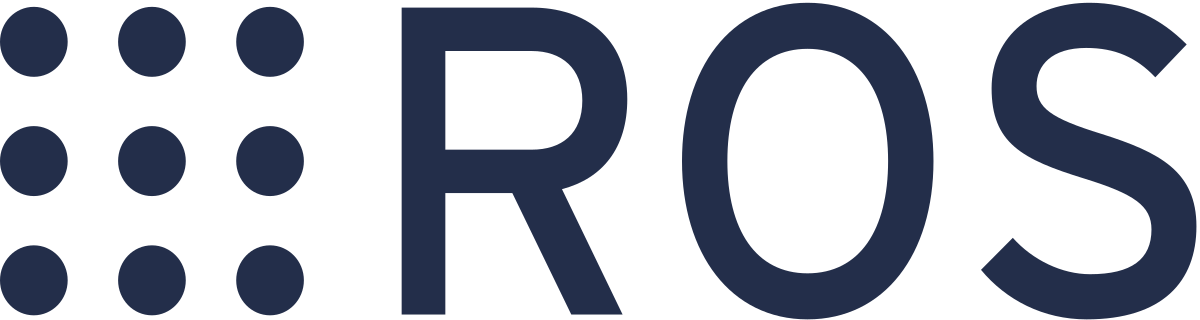
\includegraphics[width=0.7\linewidth]{Images/logos/ros}
			\label{fig:ros}
		\end{figure}

		
			The first decission we had to make was about the architecture of the project. Was it a good idea to build all the project in the same computer? How should we communicate with the Robot?

		We found the best solution for this questions in ROS (Robot Operative System), which is a framework for the development of software for robots that provides the functionality of an operating system in a heterogeneous cluster. ROS was originally developed in 2007 under the name switchyard by the Stanford Artificial Intelligence Laboratory to support the Stanford Artificial Intelligence Robot (STAIR) project. Since 2008, development has continued primarily at Willow Garage, a robotic research institute with more than twenty institutions collaborating on a federated development model.

		ROS provides the standard services of an operating system such as hardware abstraction, low-level device control, implementation of commonly used functionality, message passing between processes, and package maintenance. It is based on a graph architecture where the processing takes place in the nodes that can receive, send and multiplex messages from sensors, control, states, schedules and actuators, among others. The library is oriented for a UNIX system (Ubuntu (Linux)) although it is also adapting to other operating systems such as Fedora, Mac OS X, Arch, Gentoo, OpenSUSE, Slackware, Debian or Microsoft Windows, considered as 'experimental'.
		ROS is free software under BSD license terms. This license allows freedom for commercial and investigative use. Contributions of packages in ros-pkg are under a variety of different licenses.

		All of these features made ROS ideal for the project. Specially the following ones:
		\begin{itemize}
			\item[\textendash]Universal Robots drivers for ROS using mooveit make it possible to controll ROS remotelly.
			\item[\textendash] ROS is a multi-node oriented framework, which allows us to take all the advantages of micro-services. We can split the software by functionallity gaining:
			\begin{itemize}
				\item[\textendash]The possibility of giving more or less computation power to each functionality depending on its needs. In the project we have useed from  computers with the better Nvidia Graphic card and 32 GB of RAM to other mini-computers such as a Raspberry-pi or an Arduino Card.
				\item[\textendash]The chance of using a different environment for each functionality. Different versions of python and even different programming languages, diferent versions of libraries, diferent Operative Systems, etc.
				\item[\textendash]Isolation of each component of the project, allowing us to develop separatly each functionality without affecting the rest of the functionalities of the project.
			\end{itemize}
			\item[\textendash]It can work over an Arduino Card. It is not self sufficient, as it needs to be serial connected to a computer (Or Raspberry pi) in orther to work. We needed the arduino card in order to build our "home made" vaccuum gripper.
			\item[\textendash]It is open source and have a huge community, so we could reuse some already developed solutions such as the usb\_cam package, which let us take pictures from a camara connected to another node or computer.
			
		\end{itemize}


	\section{pytorch}
	
		\begin{figure}[h!]
			\centering
			
\includegraphics[width=0.7\linewidth]{Images/logos/pytorch}
			\label{fig:pytorch}
		\end{figure}
	
		PyTorch is a Python package designed to perform numerical calculations using tensor programming. It also allows its execution on GPU to speed up calculations.
	
		Typically PyTorch is used both to replace numpy and process calculations on GPUs and for research and development in the field of machine learning, mainly focused on the development of neural networks. In this case we will use PyTorch in both the Reinforcement Learning algorithm and the image Processing.
	
		PyTorch is a very recent library and despite this it has a large number of manuals and tutorials where to find examples. In addition to a community that grows by leaps and bounds.
		
		PyTorch has a very simple interface for creating neural networks despite working directly with tensors without the need for a library at a higher level such as Keras for Theano or Tensorflow.
		
		Unlike other packages like Tensorflow, PyTorch works with dynamic graphs instead of static ones. This means that at runtime the functions can be modified and the calculation of the gradient will vary with them. On the other hand, in Tensorflow we must first define the computation graph and then use the session to calculate the results of the tensors, this makes it difficult to debug the code and makes its implementation more tedious.
		
		PyTorch has support to run on graphics cards (GPU), it uses internally CUDA, an API that connects the CPU with the GPU that has been developed by NVIDIA.

	\section{arduino}
		\begin{figure}[h!]
			\centering
			
\includegraphics[width=0.7\linewidth]{Images/logos/arduino}
			\label{fig:arduino}
		\end{figure}
		Arduino is an open source electronics creation platform, which is based on free hardware and software, flexible and easy to use for creators and developers. This platform allows the creation of different types of single-board microcomputers that can be used by the developer community for different types of use.

		As commented before, we will use Arduino Card in order to build a Vaccuum Gripper for the Robot. It will be connected with all the other nodes using ROS Queues.


	\section{github}
		\begin{figure}[h!]
			\centering
			
\includegraphics[width=0.7\linewidth]{Images/logos/github}
			\label{fig:github}
		\end{figure}
		GitHub, Inc. is a provider of Internet hosting for software development and version control using Git. It offers the distributed version control and source code management (SCM) functionality of Git, plus its own features. It provides access control and several collaboration features such as bug tracking, feature requests, task management, continuous integration and wikis for every project. Headquartered in California, it has been a subsidiary of Microsoft since 2018.
			
		GitHub offers its basic services free of charge. Its more advanced professional and enterprise services are commercial. Free GitHub accounts are commonly used to host open-source projects. As of January 2019, GitHub offers unlimited private repositories to all plans, including free accounts, but allowed only up to three collaborators per repository for free. Starting from April 15, 2020, the free plan allows unlimited collaborators, but restricts private repositories to 2,000 minutes of GitHub Actions per month. As of January 2020, GitHub reports having over 40 million users  and more than 190 million repositories  (including at least 28 million public repositories),  making it the largest host of source code in the world.

	\section{CUDA}
		\begin{figure}[h!]
			\centering
			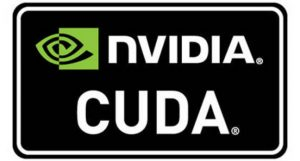
\includegraphics[width=0.7\linewidth]{Images/logos/cuda}
			\label{fig:cuda}
		\end{figure}
		CUDA stands for Compute Unified Device Architecture, which refers to a parallel computing platform including a compiler and a set of development tools created by nvidia that allow programmers to use a variation of the language. C programming for encoding algorithms on nvidia GPUs.

		Through wrappers you can use Python, Fortran and Java instead of C / C ++.
		
		Works on all nvidia GPUs from the G8X series onwards, including GeForce, Quadro, ION, and the Tesla line.1 nvidia claims that programs developed for the GeForce 8 series will also work without modification on all future nvidia cards, thanks to binary compatibility.
		
		CUDA tries to exploit the advantages of GPUs over general purpose CPUs by using the parallelism offered by its multiple cores, which allow the launch of a very high number of simultaneous threads. Therefore, if an application is designed using multiple threads that perform independent tasks (which is what GPUs do when processing graphics, their natural task), a GPU will be able to offer great performance in fields that could range from computational biology to biology. crypto, for example.
		
		The first SDK was released in February 2007 initially for Windows, Linux, and later in version 2.0 for Mac OS. It is currently offered for Windows XP / Vista / 7/8/102, for Linux 32/64 bits3 and for macOS4.

	\section{moveit}
		\begin{figure}[h!]
			\centering
			
\includegraphics[width=0.7\linewidth]{Images/logos/moveit}
			\label{fig:moveit}
		\end{figure}
	
		MoveIt! is open source software for ROS (Robot Operating System) which is state of the art software for mobile manipulation. In fact, we could say that MoveIt! it is becoming a de facto standard in the field of mobile robotics, as today more than 65 robots use this software, including the latest robots developed by Robotnik.
		
		MoveIt! includes various utilities that speed up the work with robotic arms, and it helps to not be continually “reinventing the wheel”, following the ROS philosophy of code reuse.
		
	\section{Universal Robots driver for ROS}	
		\begin{figure}[h!]
			\centering
			
\includegraphics[width=0.7\linewidth]{Images/logos/ur}
			\label{fig:ur}
		\end{figure}
	
	
		Universal Robots have become a dominant supplier of lightweight, robotic manipulators for industry, as well as for scientific research and education. The Robot Operating System (ROS) has developed from a community-centered movement to a mature framework and quasi standard, providing a rich set of powerful tools for robot engineers and researchers, working in many different domains.
		
		With the release of UR’s new e-Series, the demand for a ROS driver that supports the new manipulators and the newest ROS releases and paradigms like ROS-control has increased further. The goal of this driver is to provide a stable and sustainable interface between UR robots and ROS that strongly benefit all parties.
	
	
	\section{UR3 robot}
	
		% TODO: Definir el número de motores independientes del robot y los tipos de coordenadas y movimientos que se pueden hacer con él
	
		The UR3 Universal Robots robot is the smallest cobot of the UR series of Universal. Universal Robots' ultra flexible UR3 provides high precision for the smallest production environments.
		
		\begin{figure}[h!]
			\centering
			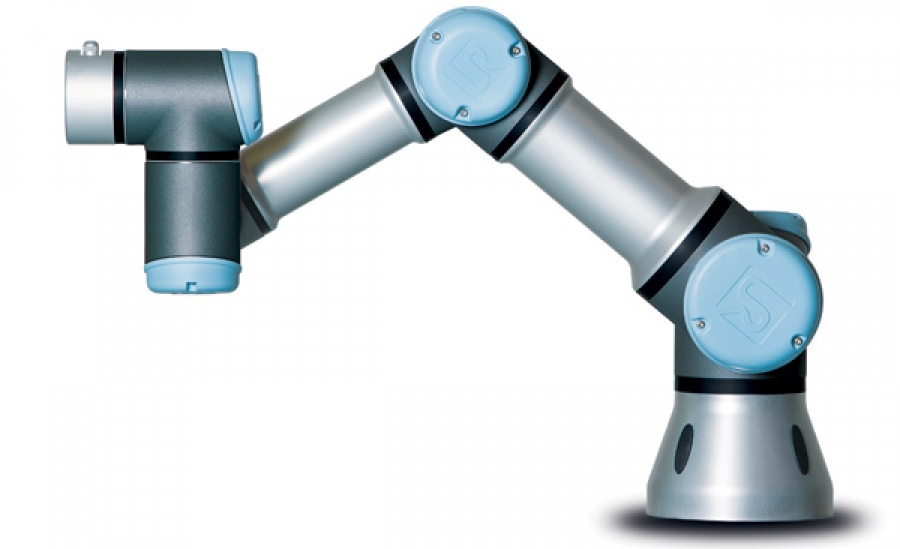
\includegraphics[width=0.7\linewidth]{Images/logos/ur3}
			\label{fig:ur3}
		\end{figure}
	
		
		It can modulate payloads of up to 3 kg, adding value to scientific, pharmaceutical, agricultural, electronic and technological facilities. Tasks the UR3 excels at include: mounting small objects, gluing, screwing, tool handling, welding and painting.
		
		However, the range of movements of this robot is really limited, and it can only lift up 3 Kilograms so this robot is really good for preparing a prototype, it has the same characteristics than its big brothers, but probably it is not good enough to build a production solution.	
		
	\section{anaconda}
		\begin{figure}[h!]
			\centering
			
\includegraphics[width=0.7\linewidth]{Images/logos/anaconda}
			\label{fig:anaconda}
		\end{figure}
		Anaconda is a free and open distribution of the Python and R languages, used in data science, and machine learning. This includes processing of large volumes of information, predictive analytics and scientific computations. It is aimed at simplifying the deployment and management of software packages.
		
		The different versions of the packages are managed through the conda package management system, which makes it quite easy to install, run, and update data science and machine learning software such as Scikit-team, TensorFlow and SciPy.
		
		The Anaconda distribution is used by 6 million users and includes more than 250 data science packages valid for Windows, Linux, and MacOS.

	
